\documentclass{article}
\usepackage{lipsum}
\usepackage{authblk}
\usepackage{listings}
\usepackage{xcolor}
\usepackage{hyperref}
\usepackage{tikz}
\usepackage{graphicx}
\usetikzlibrary{shapes.geometric, arrows}
\usepackage[utf8]{inputenc}
\usepackage{subcaption}
\usepackage{caption}
\usepackage{amssymb}
\usepackage{amsmath}
\usepackage[a4paper,total={7in, 8in}]{geometry}
% \usepackage[hidelinks]{hyperref} % Commented out to avoid option clash
\usepackage{bm}
\usepackage{centernot}
\usepackage{titling}
\usepackage{color}
\usepackage{listings}
\usepackage{graphicx} % Required for inserting images
\usepackage{tikz}
\tikzstyle{mybox} = [draw=black, thin, rectangle, rounded corners, inner ysep=5pt, inner xsep=5pt, fill=orange!20]


%Per disegnare il box
%\hspace*{-5mm}
%\begin{tikzpicture}
%\node [mybox] (box){%
%    \begin{minipage}{.96\textwidth}     %Larghezza del box
            %Qui testo
%    \end{minipage}
%};
%\end{tikzpicture}%


\usepackage{tcolorbox}
\tcbuselibrary{listingsutf8} % Per supportare codice e stili terminal-like
% Stili per i nodi e le frecce
\tikzstyle{block} = [rectangle, minimum width=2.5cm, minimum height=1cm, text centered, draw=black]
\tikzstyle{run1} = [block, fill=red!40]
\tikzstyle{run2} = [block, fill=blue!40]
\tikzstyle{run3} = [block, fill=green!40]
\tikzstyle{arrow} = [thick,->,>=stealth]

\title{\textbf{[Manuale Utente] Realizzazione di un ambiente di fault injection per applicazione ridondata}}

\author{Carlo Migliaccio}
\author{Federico Pretini}
\author{Alessandro Scavone}
\author{Mattia Viglino}
\affil[1]{\small{Laurea Magistrale in Ingegneria Informatica, Politecnico di Torino}}

\date{Gennaio 2025}

\pagestyle{headings}

\begin{document}

\counterwithin{figure}{section}
\counterwithin{equation}{section}
\renewcommand{\labelenumii}{\arabic{enumi}.\arabic{enumii}}

\maketitle
\thispagestyle{empty}
\vspace{-0.8cm}
\tableofcontents

\section*{Introduzione}
Questo manuale fornisce istruzioni rapide per utilizzare il programma scritto in Rust. \\
Un menu interattivo consente di personalizzare l'esecuzione della pipeline di fault injection, scegliendo i dati di input, l'algoritmo di esecuzione e il tipo di report generato.

\section*{Requisiti}
\begin{itemize}
\item \textbf{Sistema operativo}: macOS, Linux o Windows.
\item \textbf{Compilatore Rust}: \texttt{rustc} installato. Puoi installarlo da \url{https://rustup.rs}.
\end{itemize}

\section*{Come Aprire ed Eseguire il Programma}
\begin{enumerate}
\item Accedi alla stessa directory che contiene il file \texttt{Cargo.toml} del progetto.
\item Esegui il programma con il comando \texttt{cargo run}.
\end{enumerate}

\section*{Guida al Menù}
\subsection{Come navigare nel menu}
Dopo l'avvio, il programma presenterà un menu interattivo.\\
La \textbf{scelta corrente} è evidenziata dall'indicatore visivo \texttt{>}.\\
Per navigare tra le opzioni del menu, utilizza i tasti freccia \textbf{Su} e \textbf{Giù}.\\
Premere il tasto \textbf{Invio} per confermere la selezione. \\ 
Una selezione predefinita è racchiusa tra parentesi quadre \textbf{[default option]}, per cofermarla premere \textbf{Invio}.

\subsection{Scelte del menù}
Il menù del programma ti permetterà di eseguire la pipeline di fault injection in maniera personalizzata.\\
Di seguito vengono descritti gli step passo passo.

\paragraph{Passo 1: Inserisci il nome del file per il report.}\leavevmode\\
All'avvio, il programma richiede di specificare il nome del file per il report, il documento pdf generato al termine dell'analisi con i risultati più importanti.
Il nome del file può essere digitato da tastiera, non deve contenere l'estensione e consente solamente numeri, lettere, - e \_.
L'opzione [report] rappresenta il nome di default.\\ \\
Esempio passo 1:
\begin{tcolorbox}[colback=black,coltext=white,sharp corners,boxrule=0.5mm,width=\textwidth]
---------------------------------------------------------------------------------------------------\\
 Realizzazione di un ambiente di Fault Injection per applicazione ridondata \\
 ---------------------------------------------------------------------------------------------------\\

Inserisci il nome del file per il report SENZA ESTENSIONE [report]:
\end{tcolorbox}

\paragraph{Passo 2: Scegli la sorgente dei dati.}\leavevmode\\
La sorgente dei permette di specificare il vettore sui cui verrano applicati gli algoritmi di ordinamento e le due matrici che verrano moltiplicate tra loro.
\begin{itemize}
    \item \textbf{Data file} \\Il data file è un file di input personalizzabile con precaricati un vettore randomico, la matrice di Wilson e la sua inversa. Il file è disponibile al percorso src/data/input.txt.
    \item \textbf{Dataset} \\ Il dataset è una cartella sorgente composta da due file. \\Il primo file contiene vettori casuali a dimensioni variabili.\\ 
    Il secondo file contiene 64 matrici di rotazione 3x3. \\
    Se viene eseguita un'analisi con algortimo matrix multiplication (prossimo passo), una di queste matrici verrà presa randomicamente e scalata con una matrice di scalamneto uniforme randomica.
\end{itemize}
Esempio passo 2:
\begin{tcolorbox}[colback=black, coltext=white, sharp corners, boxrule=0.5mm, width=\textwidth]
    Seleziona la sorgente dei dati: \\
    \texttt{>} Data file \\
    \hspace{2.5em}Dataset
\end{tcolorbox}


\paragraph{Passo 3: Seleziona il tipo di analisi.}\leavevmode\\
In entrambi i casi (\textit{Data file} o \textit{Dataset}), è possibile scegliere tra:
\begin{itemize}
    \item \textbf{Singolo algoritmo}: Esegue la pipeline di fault injection su un singolo algoritmo.
    \item \textbf{Tutti gli algoritmi}: Esegue la pipeline di fault injection sequenzialmente per tutti gli algoritmi disponbili.
\end{itemize}
Esempio passo 3:
\begin{tcolorbox}[colback=black, coltext=white, sharp corners, boxrule=0.5mm, width=\textwidth]
    Seleziona il tipo di analisi: \\
    \texttt{>} Esegui un singolo algoritmo \\
    \hspace{2.5em}Esegui un'analisi comparativa tra tutti gli algoritmi
\end{tcolorbox}


\paragraph{Passo 4: Configura l'algoritmo (se  scelto \textit{Singolo algoritmo}).}\leavevmode\\
Se è stata selezionata l'opzione \textit{Singolo algoritmo}, sarà necessario scegliere un algoritmo tra:
\begin{itemize}
    \item \textbf{Selection Sort}: algortimo di ordinamento per un vettore.
    \item \textbf{Bubble Sort}: algortimo di ordinamento per un vettore.
    \item \textbf{Matrix multiplucation}: moltiplicazione tra matrici quadrate.  
\end{itemize}
Esempio passo 4:
\begin{tcolorbox}[colback=black, coltext=white, sharp corners, boxrule=0.5mm, width=\textwidth]
    Scegli un algoritmo da utilizzare: \\
    \texttt{>} Selection Sort \\
    \hspace{2.5em}Bubble Sort \\
    \hspace{2.5em}Matrix Multiplication
\end{tcolorbox}


\paragraph{Passo 5: Configura la modalità .}\leavevmode\\ \leavevmode\\
Se \textbf{Singolo:}\\
Dopo aver scelto l'algoritmo, si accede alla configurazione della modalità. Sono disponibili le seguenti opzioni:
\begin{itemize}
    \item \textbf{Cardinalità a piacere della fault entry}\\Esegue l'analisi per l'algoritmo precedentemente selezionato una sola volta con le entry selezionate da tastiera.\\ L'opzione [2000] rappresenta la cardinalità di default.
    \item \textbf{Cardinalità 1000, 2000, 3000}\\Esegue l'analisi per l'algoritmo precedentemente selezionato tre volte per le cardinalità della fault list 1000, 2000 e 3000.
\end{itemize}
Esempio passo 5.1:
\begin{tcolorbox}[colback=black, coltext=white, sharp corners, boxrule=0.5mm, width=\textwidth]
    Scegli una modalità di single analysis: \\
    \texttt{>} Digita una cardinalità a piacere per la fault list entry\\
    \hspace{2.5em}Tre esecuzioni con cardinalità della fault list entry che varia 11000, 2000, 3000] \\
\end{tcolorbox}
Se \textbf{Tutti:}\\
Nel caso in cui sia stata selezionata l'opzione \textit{Tutti gli algoritmi}, la modalià è predefinita ma si può modificare:
\begin{itemize}
\item \textbf{Cardinalità a piacere della fault entry}\\Esegue tutti gli algoritmi sequenzialmente con le entry selezionate da tastiera.\\ L'opzione [2000] rappresenta la cardinalità di default.
\end{itemize}
Esempio passo 5.2:
\begin{tcolorbox}[colback=black, coltext=white, sharp corners, boxrule=0.5mm, width=\textwidth]
    Inserisci il numero di fault entries desiderate [2000]: 
\end{tcolorbox}

\paragraph{Passo 6: Avvio dell'analisi.}\leavevmode\\
Confermando l'ultima scelta la pipeline di fault injection verrà eseguita con i parametri selezionati.\\
Una volta completata l'analisi, viene mostrato il messaggio \textit{"operazione completata"} e verrà salvato il report nella cartella results. \\
In base alla configurazione scelta, il report sarà di diverso tipo:
\begin{itemize}
    \item Se è stata selezionata l'opzione \textit{Singolo algoritmo} e \textit{Cardinalità a piacere della fault entry}, verrà generato un report con nome \texttt{[nomefile].pdf}.
    \item Se è stata selezionata l'opzione \textit{Singolo algoritmo} e \textit{Cardinalità 1000, 2000, 3000}, verrà generato un report comparativo con nome \texttt{[nomefile]\_diffcard.pdf}.
    \item Se è stata selezionata l'opzione \textit{Tutti gli algoritmi}, verrà generato un report comparativo con nome \texttt{[nomefile]\_all.pdf}.
\end{itemize}

\subsection{Diagramma della struttura del menu}
Di seguito viene riportato un diagramma esplicativo della struttura del menu.\\ \\ \\
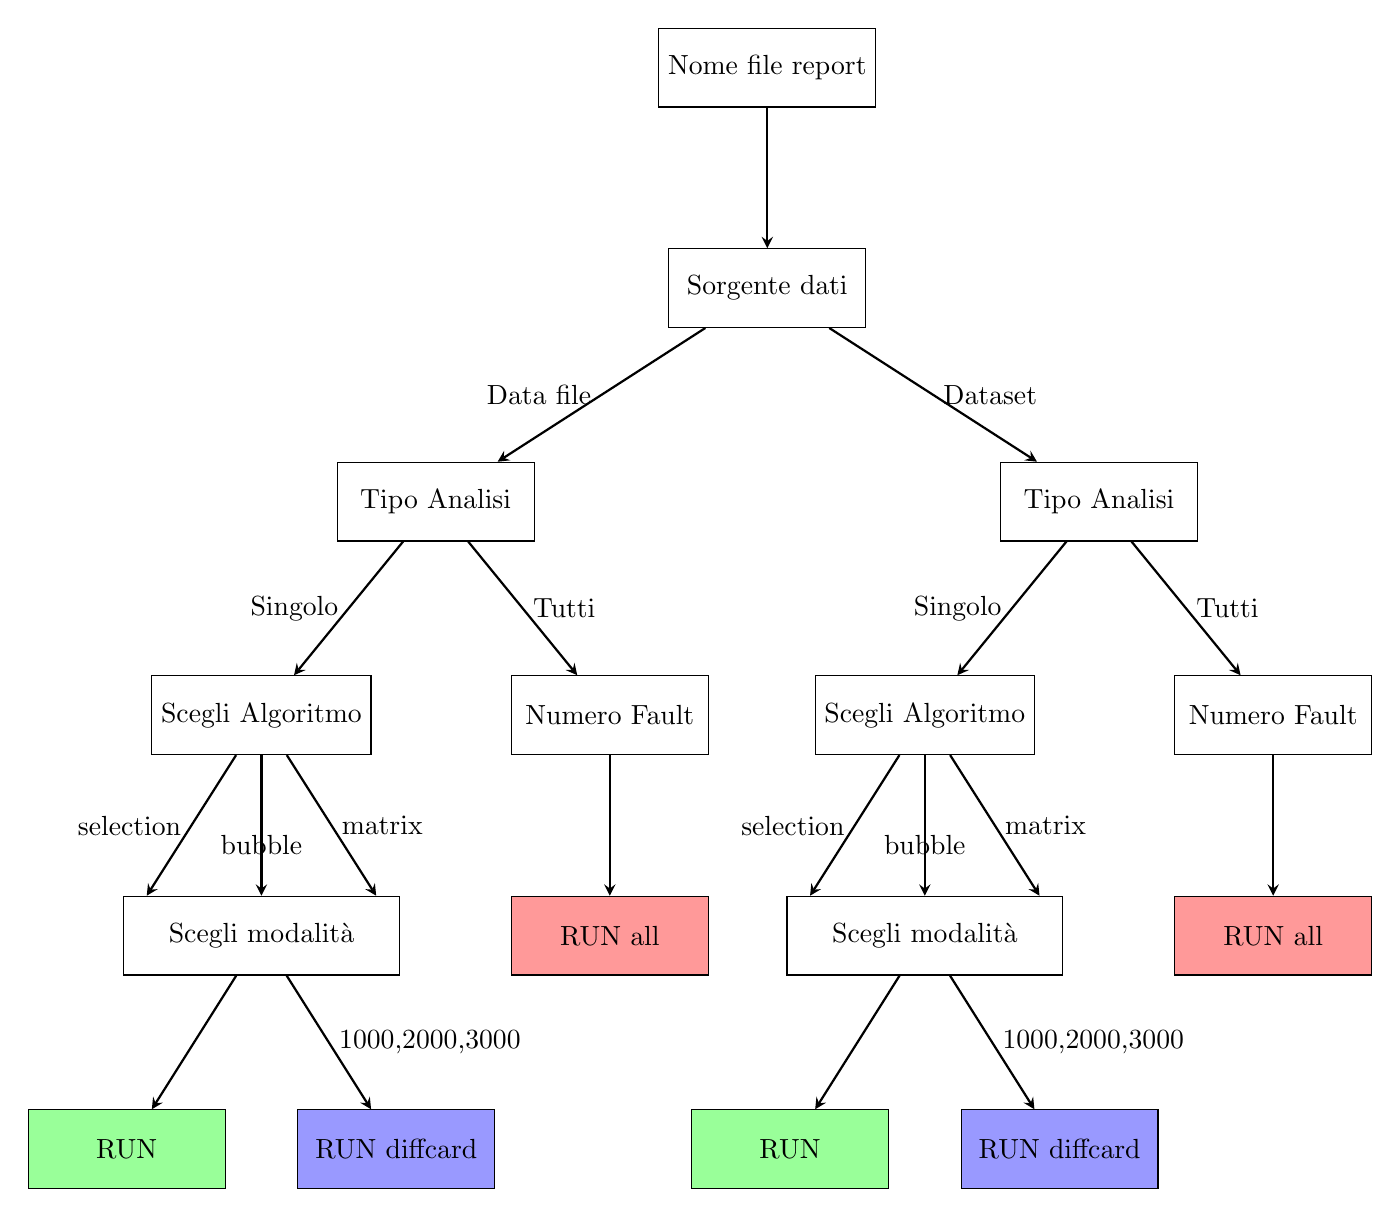
\begin{tikzpicture}[node distance=0.3cm]
% Nodi principali
\node (fileinput) [block] {Nome file report};

\node (datasource) [block, below of=fileinput, yshift=-2.5cm] {Sorgente dati};

\node (analysis1) [block, below left of=datasource, yshift=-2.5cm, xshift=-4cm] {Tipo Analisi};
\node (analysis2) [block, below right of=datasource, yshift=-2.5cm, xshift=4cm] {Tipo Analisi};

\node (algorithm1) [block, below left of=analysis1, yshift=-2.5cm, xshift=-2cm] {Scegli Algoritmo};
\node (numfault1) [block, below right of=analysis1, yshift=-2.5cm, xshift=2cm] {Numero Fault};
\node (algorithm2) [block, below left of=analysis2, yshift=-2.5cm, xshift=-2cm] {Scegli Algoritmo};
\node (numfault2) [block, below right of=analysis2, yshift=-2.5cm, xshift=2cm] {Numero Fault};


\node (modalita1) [rectangle, draw, minimum width=3.5cm, minimum height=1cm,below  of=algorithm1, yshift=-2.5cm] {Scegli modalità};
\node (run1) [run1, below of=numfault1, yshift=-2.5cm] {RUN all};
\node (modalita2) [rectangle, draw, minimum width=3.5cm, minimum height=1cm,below  of=algorithm2, yshift=-2.5cm] {Scegli modalità};
\node (run2) [run1, below of=numfault2, yshift=-2.5cm] {RUN all};

\node (run5) [run3, below left of=modalita1, yshift=-2.5cm, xshift=-1.5cm] {RUN};
\node (run3) [run2, below right of=modalita1, yshift=-2.5cm, xshift=1.5cm] {RUN diffcard};
\node (run6) [run3, below left of=modalita2, yshift=-2.5cm, xshift=-1.5cm] {RUN};
\node (run4) [run2, below right of=modalita2, yshift=-2.5cm, xshift=1.5cm] {RUN diffcard};



% Frecce e testi sulle connessioni
\draw [arrow] (fileinput) -- (datasource) node[midway, right] {};

\draw [arrow] (datasource) -- (analysis1) node[midway, left] {Data file};
\draw [arrow] (datasource) -- (analysis2) node[midway, right] {Dataset};

\draw [arrow] (analysis1) -- (algorithm1) node[midway, left] {Singolo};
\draw [arrow] (analysis1) -- (numfault1) node[midway, right] {Tutti};
\draw [arrow] (analysis2) -- (algorithm2) node[midway, left] {Singolo};
\draw [arrow] (analysis2) -- (numfault2) node[midway, right] {Tutti};

\draw [arrow] (algorithm1) -- node[midway, left] {selection} ([xshift=3mm, yshift=0mm]modalita1.north west);
\draw [arrow] (algorithm1) -- node[midway, below] {bubble} (modalita1.north);
\draw [arrow] (algorithm1) -- node[midway, right] {matrix} ([xshift=-3mm, yshift=0mm]modalita1.north east);
\draw [arrow] (numfault1) -- (run1) node[midway, right] {};
\draw [arrow] (algorithm2) -- node[midway, left] {selection} ([xshift=3mm, yshift=0mm]modalita2.north west);
\draw [arrow] (algorithm2) -- node[midway, below] {bubble} (modalita2.north);
\draw [arrow] (algorithm2) -- node[midway, right] {matrix} ([xshift=-3mm, yshift=0mm]modalita2.north east);
\draw [arrow] (numfault2) -- (run2) node[midway, right] {};

\draw [arrow] (modalita1) -- (run5) node[midway, left,align=center] {};
\draw [arrow] (modalita1) -- (run3) node[midway, right, align=center] {1000,2000,3000};
\draw [arrow] (modalita2) -- (run6) node[midway, left,align=center] {};
\draw [arrow] (modalita2) -- (run4) node[midway, right, align=center] {1000,2000,3000};


\end{tikzpicture}

\subsection{Esempio di utilizzo}
Di seguito viene riportato un esempio completo di esecuzione con sorgente da data file per tutti gli algortimi con 2000 fault entries.\\
\textbf{Scelte del menù:}\\
\begin{tcolorbox}[colback=black, coltext=white, sharp corners, boxrule=0.5mm, width=\textwidth]
---------------------------------------------------------------------------------------------------\\
 Realizzazione di un ambiente di Fault Injection per applicazione ridondata \\
---------------------------------------------------------------------------------------------------\\ \\
Inserisci il nome del file per il report SENZA ESTENSIONE: report\\
Seleziona la sorgente dei dati: Data file\\
Seleziona il tipo di analisi: Esegui un'analisi comparativa tra tutti gli algoritmi\\
Inserisci il numero di fault entries desiderate: 2000\\
Esecuzione Selection Sort\\
Esecuzione Bubble Sort\\
Esecuzione Matrix Multiplication\\
Operazione completata. Report salvato in: results/report\_all.pdf\\
\end{tcolorbox}
\textbf{Report PDF di output:}\\

\end{document}
